\section{Datum WGS84 DAN NAD83}
\subsection{Pengertian DATUM}

Datum merupakan sebuah istilah yang dicetuskan oleh Alfred North Whitehead untuk menunjukan berbagai varian informasi yang dimiliki oleh entitas aktual. Di dalam sistem filsafat proses, datum dapat diperoleh melalui peristiwa konkresi. Setiap entitas aktual memiliki berbagai macam datum. Saat entitas aktual sudah mencapai kepenuhannya, satisfaction, ia akan mengalami peristiwa yang biasa disebut konkresi. Peristiwa inilah yang membuat entitas aktual memberikan informasi-informasi bagi potensi terbentuknya entitas aktual lainnya. Informasi-informasi inilah yang disebut dengan datum. Di dalam setiap peristiwa prehensi datum dapat diterima sebagai potensi informasi yang relevan dalam pembentukan entitas aktual dan datum dapat ditolak berdasarkan pertimbangan relevansi entitas aktual yang akan terbentuk. Proses diterimanya datum sebagai informasi relevan dari entitas aktual lainnya melalui peristiwa prehensi yang disebut sebagai prehensi positif. Proses ditolaknya datum sebagai informasi relevan dari entitas aktual lainnya melalui peristiwa prehensi yang disebut sebagai prehensi negatif.
Satu potensi entitas aktual merasakan banyak datum dari berbagai entitas aktual yang ada di dalam semesta. Ketika entitas aktual hendak mewujudkan dirinya, ia akan merasakan banyak datum. Datum yang dirasakan oleh entitas aktual merupakan datum-datum yang telah mengalami proses penolakan dan proses penerimaan yang panjang di dalam ruang dan waktu oleh entitas aktual melalui prehensi. Datum yang diterima sebagai informasi yang relevan bagi suatu potensi terbentuknya entitas aktual yang baru, merupakan datum yang telah mengalami proses ditolak dan diterima melalui prehensi oleh entitas aktual sebelumnya. Datum yang lahir dari peristiwa konkresi merupakan datum-datum yang khas dan baru. Datum yang satu berbeda dengan datum yang lainnya. Sebuah entitas aktual terdiri dari berbagai macam datum. Datum-datum ini terbentuk secara unik melalui peristiwa konkresi.
Datum geodetik atau referensi permukaan atau georeferensi merupakan parameter yang digunakan sebagai acuan untuk mendefinisikan geometri ellipsoid bumi. Datum geodetik diukur menggunakan metode manual hingga metode yang memiliki akurasi yang lebih akurat, yakni menggunakan satelit.

\begin{table}[h]
\caption{Ellipsoid Geosentrik WGS84}
\centering
\begin{tabular}{p{1.25in}p{1.25in}p{1.25in}}
\hline
Parameter&Notasi&Nilai\\
\hline
Sumbu Panjang & a & 6378137 m\\
Penggepengan & f & 1/298.257223563\\
Kecepatan Sudut Bumi & w & 7292115.0 x 10$^{-11}$ rad s$^{-1}$\\
Konstanta Gravitasi Bumi ( termasuk massa atmosfernya ) & GM & 3986004.418 x 108 m$^3$$ s^{-2}$\\
\hline
\end{tabular}
\label{table:contoh}
\end{table}

Dibawah ini merupakan Jenis geodetik menurut metodenya :
\begin{enumerate}
\item Datum horizontal adalah datum yang digunakan untuk pemetaan horisontal. Dengan teknologi yang lebih maju, kini muncul tren penggunaan datum horizontal dari koordinat geosentris global sebagai penggganti datum lokal atau regional.
\begin{figure}[htbp]
		\centering
		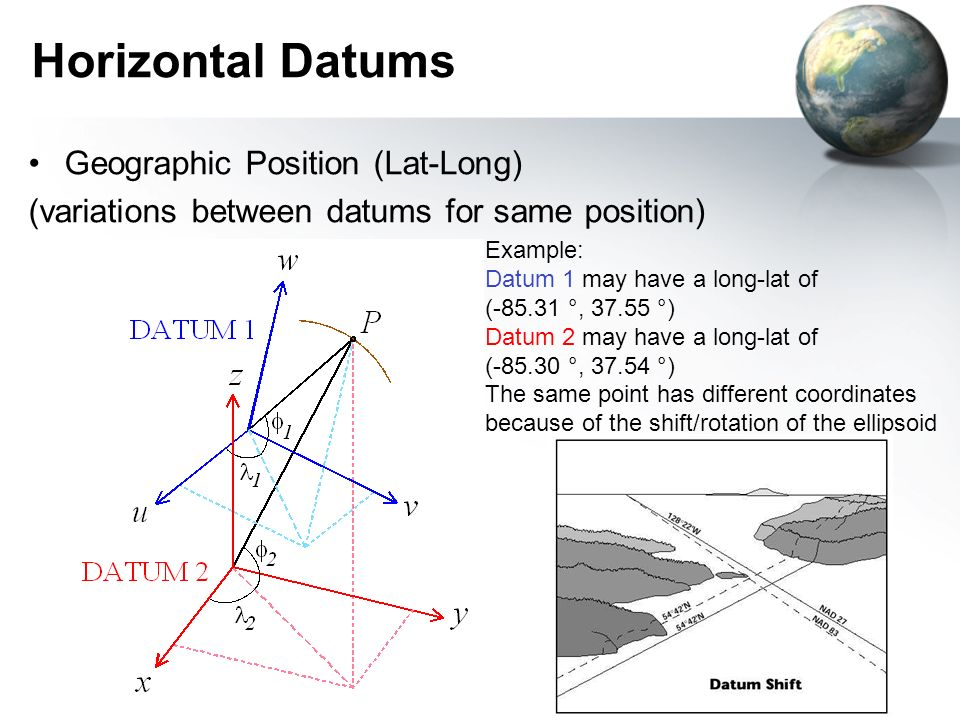
\includegraphics[width=0.75\textwidth]{pictures/datum_horizontal.jpg}
		\caption{Datum Horizontal (Sumber : https://www.slideshare.net/AeroMetri)}
		\label{Datum Horizontal}
		\end{figure}	

\item Datum vertikal adalah sistem referensi untuk ortometris medan tinggi. Datum vertikal digunakan untuk mewakili ketinggian atau kedalaman informasi. Biasanya bidang referensi yang digunakan untuk ortometris sistem tinggi adalah geoid.
\begin{figure}[htbp]
		\centering
		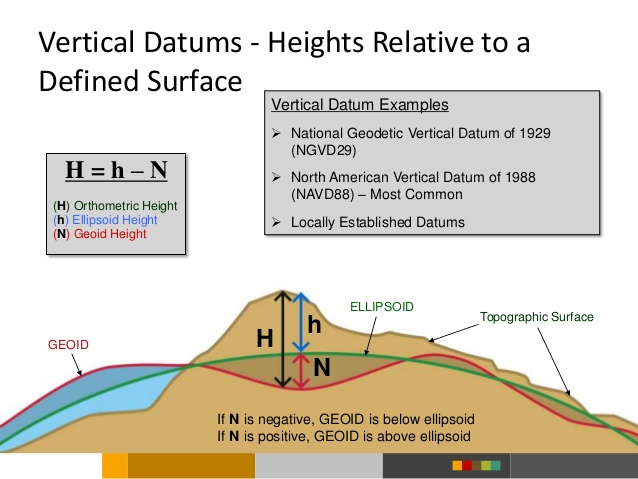
\includegraphics[width=0.75\textwidth]{pictures/vertical_datum.jpg}
		\caption{Datum Vertikal (Sumber : Map Projections and Coordinate Systems 2014)}
		\label{Datum Vertikal}
		\end{figure}	
\end{enumerate}